\subsubsection{\texttt{RN-4}: documentación de API REST}
\label{subsec:rn4}

Con la misma vocación de mantenibilidad que el requisito \texttt{RN-2} ---detallado en la \referenciaSeccion{subsec:rn2}---, el presente requerimiento busca potenciar la documentación del proyecto \textit{VSCode4Teaching}, entendiendo que este es uno de los pilares esenciales que permite a todos los desarrolladores ---con independencia de si pertenecen al proyecto o no--- comprender de forma sencilla y ágil el funcionamiento de la aplicación y la organización y aspecto del código fuente que lo conforma.

La API REST es el ``eje vertebrador'' que da unidad a \textit{VSCode4Teaching}, tal como se evidencia en la \referenciaSeccion{sec:diseñoArquitectura}, que introduce una disquisición exhaustiva sobre la organización de la aplicación que manifiesta, entre otros rasgos significativos, que esta API es la que permite la comunicación e interacción entre el servidor y los clientes de la aplicación, siendo el canal de comunicación de información bidireccional establecido entre los citados componentes.

Con el fin de potenciar la documentación existente en el proyecto sobre esta API, se ha introducido \textit{Swagger}, que es una tecnología que permite ``simplificar el desarrollo de APIs para usuarios, equipos y corporaciones con una plataforma de código abierto'' \cite{rn4_swagger}, que toma las declaraciones de \textit{endpoints} disponibles en el código fuente del servidor para generar su documentación automáticamente en el formato estipulado en el estándar \textit{OpenAPI}, que fue creado por un ``consorcio de [...] expertos que reconoce el inmenso valor de estandarizar cómo se describen las APIs''\cite{rn4_openapi} y que es uno de los más extendidos en la actualidad. Adicionalmente, permite la visualización gráfica de la documentación generada en un entorno intuitivo a través de cualquier navegador web haciendo uso de la herramienta \textit{Swagger UI} \cite{rn4_swaggerui}, tal como puede visualizarse en la \referenciaFigura{fig:reqn4-1}. Gracias a la incorporación de esta herramienta, se introduce en el código fuente del servidor la documentación en formato JSON según el estándar \textit{OpenAPI} de la API REST implementada, viéndose actualizado concordantemente con la modificación o ampliación de la implementación de los \textit{endpoints} que integran la API de este servidor.

\begin{figure}[ht]
    \centering
    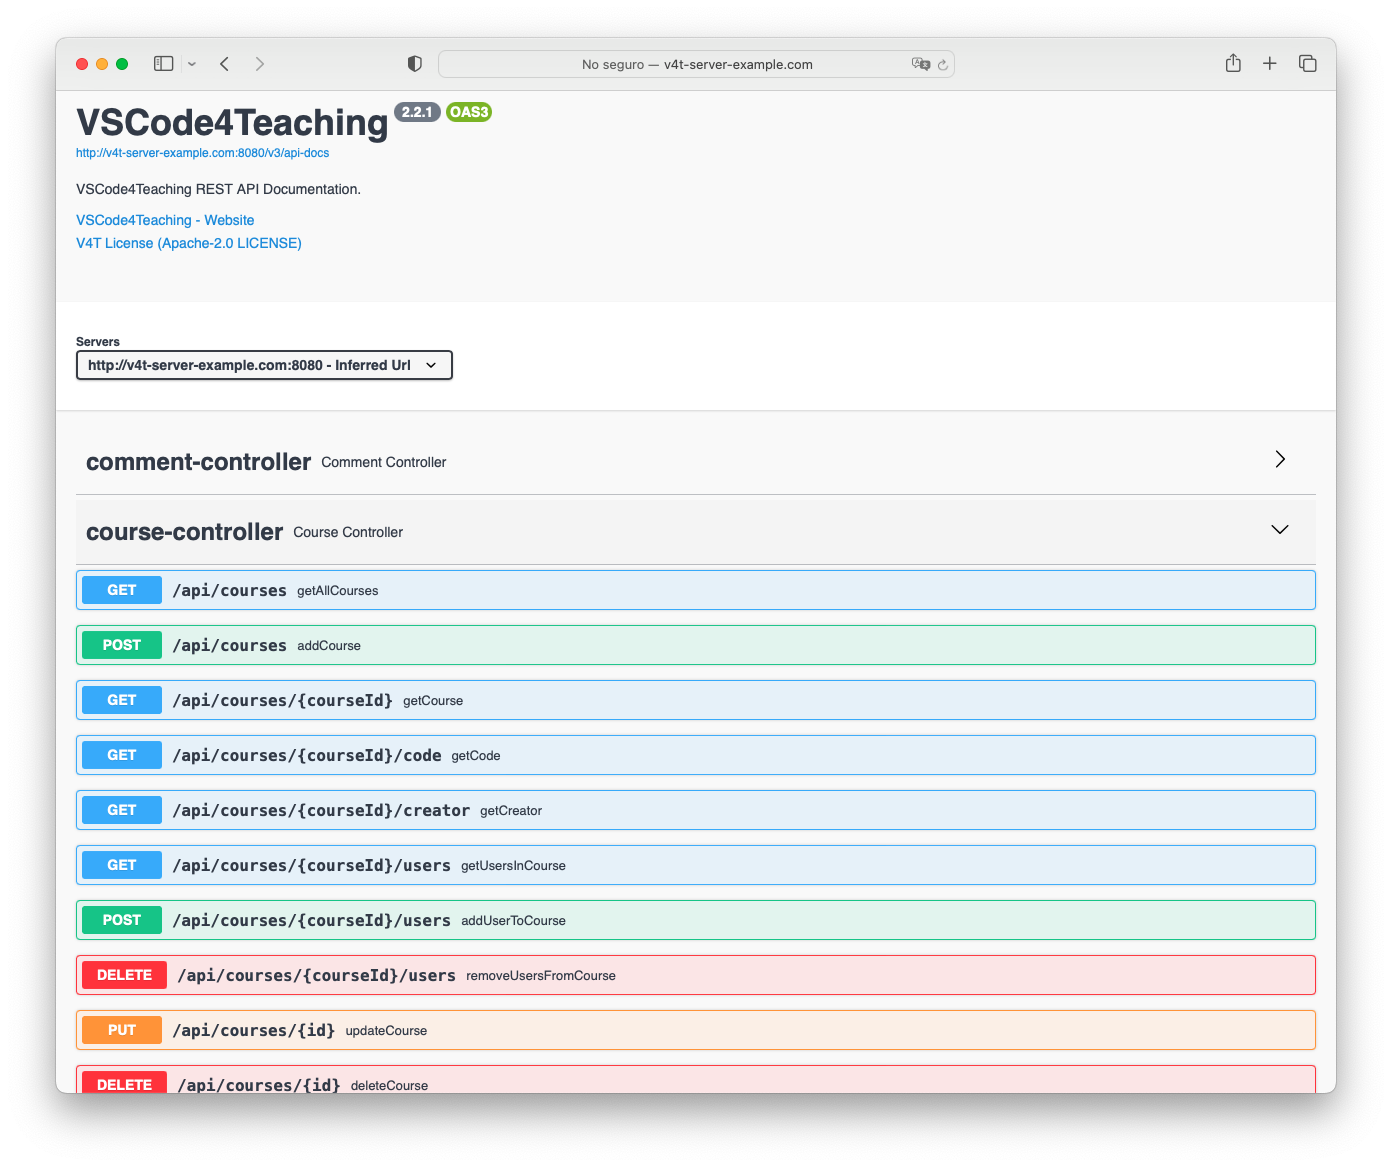
\includegraphics[width=\textwidth]{imagenes/utilizadas/4-3-implementacion/rn4-1.png}
    \caption{Vista de \textit{Swagger UI} mostrando los \textit{endpoints} disponibles en la API de VSCode4Teaching en un navegador web.}
    \label{fig:reqn4-1}
\end{figure}
